\newpage
\section{Wprowadzenie}
DO UZUPEŁNIENIA - rsa krzywych rozmiary klucza kryptoanaliza do testowania bezpieczenstwa krzywych
\subsection{Cel pracy}
Celem tej pracy jest realizacja systemu korzystającego z koprocesora GPU,
w celu przyśpieszenia obliczeń przy
rozwiązywaniu problemu logarytmu dyskretnego na krzywej eliptycznej ECCp-79 z challange'u Certicom.
\par
Głównymi elementami stworzonego systemu
jest program klienta wykonującego część algorytmu Rho Pollarda na karcie graficznej Nvidia
z wykorzystaniem technologii CUDA i języka programowania CUDA C++,
oraz program serwera działający na CPU, odpowiedzialny za zarządzanie klientami i zbieranie wyników.

\subsection{Koncepcja}
Projekt zakłada zaimplemntowanie systemu do obliczania logarytmu dyskretnego na krzywej eliptycznej.
W celu akceleracji obliczeń wykorzystuje koprocesor jakim jest GPU. Ponieważ równoległy algorytm Rho Pollarda
zakłada architekturę w postaci klient-serwer, to na projekt składa się program pełniący rolę centralnego serwera,
oraz program kliencki wykonujący obliczenia na GPU, uruchamiany w wielu instancjach.
\par
Zarówno program serwera jak i klienta, działają w ramach jednego PC, jednak architektura pozwala na wykorzystanie
wiecej niż jednej karty graficznej w celu przyspieszenia obliczeń.
Program serwera jest zaimplementowany z wykorzystaniem języka Python i odpowiada za gromadzenie znalezionych
punktów oraz za generację nowych punktów startowych. W celu optymalnego przechowywania punktów, wykorzystuje
hash mapę w formie: (\textit{współrzędne punktu} : \textit{seed}), która pozwala na szybkie sprawdzanie czy dany punkt już został znaleziony,
oraz porównanie ziarna użytego do wygenerowania punktu początkowego.
\par
Część klienta odpowiedzialna za komunikację z serwerem,
również jest zaimplementowana w języku Python i za pomocą interfejsu ABI zleca obliczenia do programu napisanego z wykorzystaniem
CUDA C++. Zarówno program serwera jak i każdego z działających klientów, uruchamiany jest w osobnym wątku, co pozwala współbieżne szukanie kolizji i efektywne
kolejkowanie kolejnych serii obliczeń na GPU.
\par
W celu komunikacji klientów z serwerem, wykorzystywane są asynchroniczne kolejki z biblioteki standardowej Pythona.
\begin{figure}[!h]
    \centering 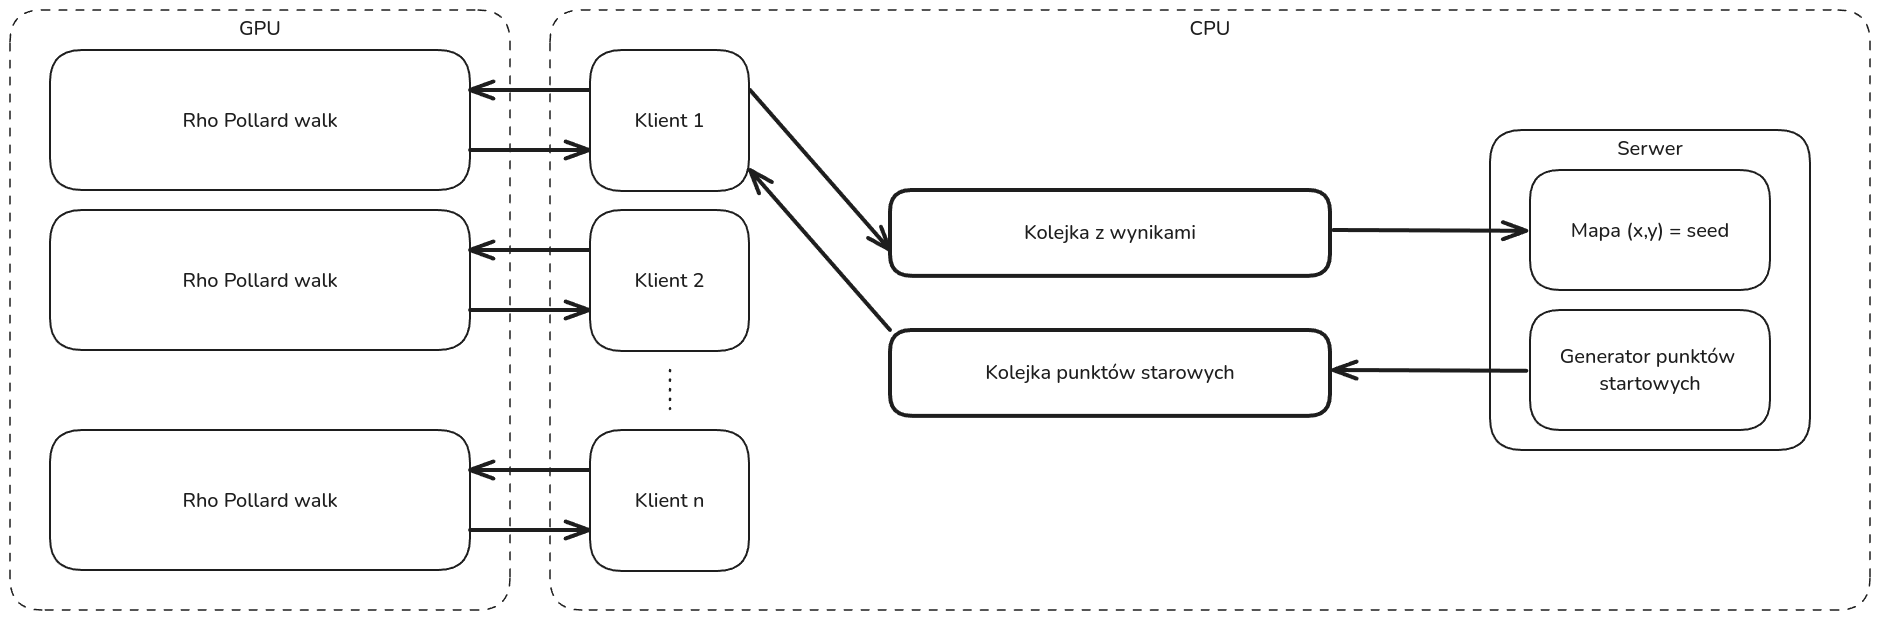
\includegraphics[width=1.1\linewidth]{arch.png}
    \caption{Schemat architektury}
\end{figure}